\documentclass[diss]{template/setrem}



\usepackage[utf8]{inputenc}
\usepackage[table]{xcolor}
\usepackage{multicol}
\usepackage{array} % for defining a new column type
\usepackage{varwidth} %for the varwidth minipage environment
\usepackage{float}
\usepackage{todonotes}
\usepackage{subfigure}
\usepackage{graphicx,url}
\usepackage{lipsum} %generate fake text

\makeatletter
\g@addto@macro{\UrlBreaks}{\UrlOrds}
\makeatother


\usepackage{setspace}
\usepackage{amssymb}
\usepackage{colortbl}
\usepackage{color}
\usepackage{hyperref}
\usepackage{verbatim}
\usepackage{scrextend}
\usepackage{csvsimple}
\usepackage{glossaries}

\usepackage{listings}
\usepackage{xcolor}
\usepackage{threeparttablex}
\usepackage{lscape}
\usepackage{colortbl}
\usepackage{booktabs}

% Coloca a contagem das figuras sequenciais sem considerar capítulos
\usepackage{chngcntr}
\usepackage{tabularx}
\usepackage{amsmath}
\usepackage{datatool}
\usepackage{seqsplit}
\usepackage[toc,page]{appendix}

% The package option longtable redefines the \cline macro to work around a bug in longtable
\usepackage{longtable}
\usepackage{multirow}
\usepackage{titletoc}

\makeatletter
\def\@cline#1-#2\@nil{%
  \omit
  \@multicnt#1%
  \advance\@multispan\m@ne
  \ifnum\@multicnt=\@ne\@firstofone{&\omit}\fi
  \@multicnt#2%
  \advance\@multicnt-#1%
  \advance\@multispan\@ne
  \leaders\hrule\@height\arrayrulewidth\hfill
  \cr
  \noalign{\nobreak\vskip-\arrayrulewidth}}
\makeatother


\counterwithout{figure}{chapter}
\counterwithout{table}{chapter}

\definecolor{color_keywords}{rgb}{0.0, 0.0, 0.44}
\definecolor{color_mykeyword}{RGB}{10, 100, 112}

\definecolor{myblue}{rgb}{0,0.3,0.9}
\definecolor{mygreen}{rgb}{0,0.6,0}
\definecolor{mygray}{rgb}{0.5,0.5,0.5}
\definecolor{mymauve}{rgb}{0.58,0,0.82}
\definecolor{mygray2}{rgb}{0.2,0.2,0.2}
\definecolor{mygray3}{rgb}{0.4,0.4,0.4}



\lstdefinestyle{mycode}{ %
  %backgroundcolor=\color{yellow!05},   % choose the background color; you must add \usepackage{color} or \usepackage{xcolor}
  basicstyle=\linespread{1}\small,        % the size of the fonts that are used for the code \footnotesize
  %lineskip={-1pt},
  breakatwhitespace=false,         % sets if automatic breaks should only happen at whitespace
  breaklines=true,                 % sets automatic line breaking
  captionpos=t,                    % sets the caption-position to top
  commentstyle=\color{gray!90},    % comment style
%  deletekeywords={...},            % if you want to delete keywords from the given language
  escapeinside={\%*}{*)},          % if you want to add LaTeX within your code
  extendedchars=true,              % lets you use non-ASCII characters; for 8-bits encodings only, does not work with UTF-8
  frame=l,                    % adds a frame around the code (bt,l,r) single
  keepspaces=true,                 % keeps spaces in text, useful for keeping indentation of code (possibly needs columns=flexible)
  keywordstyle=\color{black}\bf,       % keyword style
  language=C++,                     % the language of the code
 % morekeywords={input,output,parallel_activity,stream_producer},            % if you want to add more keywords to the set
  keywordstyle=[2]{\color{blue}\bf},
 % keywords=[3]{serial_in_order, parallel, pipeline, run, add_filter, task_scheduler_init},
 % keywordstyle=[3]{\color{blue!70!green}\bf},
  numbers=left,                    % where to put the line-numbers; possible values are (none, left, right)
  numbersep=5pt,                   % how far the line-numbers are from the code
  numberstyle=\tiny\color{mygray}, % the style that is used for the line-numbers
  rulecolor=\color{black},         % if not set, the frame-color may be changed on line-breaks within not-black text (e.g. comments (green here))
  showspaces=false,                % show spaces everywhere adding particular underscores; it overrides 'showstringspaces'
  showstringspaces=false,          % underline spaces within strings only
  showtabs=false,                  % show tabs within strings adding particular underscores
  stepnumber=1,                    % the step between two line-numbers. If it's 1, each line will be numbered
  stringstyle=\color{red},     % string literal style
  tabsize=1,                       % sets default tabsize to 2 spaces
  title=\lstname                   % show the filename of files included with \lstinputlisting; also try caption instead of title
}

% Negrito no título do listing
\captionsetup[lstlisting]{font={bf},labelfont=bf}

%Ajusta a contagem do listing
\AtBeginDocument{% the counter is defined later
  \counterwithout{lstlisting}{chapter}%
}
\makeatletter
\renewcommand{\l@lstlisting}[2]{%
  \@dottedtocline{1}{0em}{1.5em}{\lstlistingname\ #1}{#2}%
}
\makeatother


\title{your title here}
\author{Thielke}{Jônatas}
%optional
%\author{LastName}{FirstName}
\advisor[Dr.]{Griebler}{Dalvan}

% Place where the undergraduate thesis will be made.
\location{Três de Maio}{RS}

% Date of undergraduate thesis development/presentation.
\date{Agosto}{2019}

% Course name - defined in setremdefs.sty.
\course{\ctrc}
%\vspace{-4cm}

% Header image of the cover.

%% Sistemas de Informação
\courseheader{\silogo[1]}

%% Redes de Computadores
%\courseheader{\rclogo[1]}

%% Engenharia de Computação
%\courseheader{\eclogo[1]}

\docname{Undergraduate Thesis of Bachelor of Information Systems - Três de Maio Faculty - SETREM}

% Mostra a lista de tabelas e figuras com os prefixos corretos.
\titlecontents{table}
  [0em]
  {}
  {\tablename\enspace\thecontentslabel:\enspace\enspace}
  {}
  {\titlerule*[.5pc]{.}\contentspage}

\titlecontents{figure}
  [0em]
  {}
  {\figurename\enspace\thecontentslabel:\enspace\enspace}
  {}
  {\titlerule*[.5pc]{.}\contentspage}

\begin{document}


\maketitle
% folha de rosto
%%%%%%%%%%%%%%%%%%%%%%%%%%%%%%%%%%%%%%%%%%%%%%%%%%%%%%%%%%%%%%%%%%%%%%%%%%%%%%%%
\newpage

{
\begingroup\onehalfspacing
\noindent
\begin{center}
TERMO DE APROVAÇÃO

\vspace{1cm}
\textbf{NAME}\\
\textbf{NAME}

\vspace{1cm}
TITLE HERE
\end{center}

\noindent
Relatório aprovado como requisito parcial para obtenção do título de \textbf{Bacharel em Sistemas de Informação} concedido pela Faculdade de Sistemas de Informação da Sociedade Educacional Três de Maio, pela seguinte Banca examinadora:
\\
\\
\noindent
Orientador: Prof. Name, Dr.\\
Faculdade de Sistemas de Informação da SETREM
\\
\\
\noindent
Name, Dr. \\
Faculdade de Sistemas de Informação da SETREM
\\
\\
\noindent
Name, M.Sc. \\
Faculdade de Sistemas de Informação da SETREM
\\
\\
\noindent
Profa. Vera Lúcia Lorenset Benedetti, M.Sc.\\
Coordenação do Curso Bacharelado em Sistemas de Informação\\
Faculdade de Sistemas de Informação da SETREM.
\\
\\
\vfill
\begin{center}
Três de Maio, 08 de Agosto de 2019.
\end{center}
\endgroup
}



\begin{abstract}
\noindent The abstract goes here ...

\end{abstract}
\keyword{Information Systems}
\keyword{Deep Learning}
\keyword{Agriculture}
\keyword{Systematic Literature Review}




\begin{resumo}
\noindent 

O resumo vai aqui...


\end{resumo}

\keywordenglish{Sistemas de Informação}
\keywordenglish{Deep Learning}
\keywordenglish{Agricultura}
\keywordenglish{Revisão Sistemática da Literatura}




\begin{singlespaced}
\listoffigures
\end{singlespaced}

\begin{singlespaced}
\listoftables
\end{singlespaced}


% \listofmyequations

\begin{listofabbrv}{OR-AC-GAN} % Put the largest abbreviation.
\setstretch{1}
\item[ACM] {Association for Computing Machinery}
\item[AWS] {Amazon Web Services}
\item[IBGE] {Brazilian Institute of Geography and Statistics}
\item[IEEE] {Institute of Electrical and Electronics Engineers}
\item[IoT] {Internet of Things}
\end{listofabbrv}

% 
\tableofcontents

\chapter*{Introduction} \label{chap:intro}




\lipsum[2-4]

\cite{larcc}


According to ~\cite{larcc:intra-cloud_networking_cloudstack:PDP:17}, bla bla ...


Some authors prefere to include figures and others not~\citep{larcc:parsec_cloudstack_lxc_kvm:ISCC:2018}.


There are some undergraduate thesis developed at LARCC~\citep{larcc:dinei_nadine:TCC:17,larcc:anderson_willian:TCC:17,larcc:bruna_eduardo:TCC:13,larcc:charles_stein:TCC:18}
\chapter{Research Plan} \label{chap:ResearchPlan}




\section{Theme} \label{sec::Theme}

    Correlação de noticias com variaveis de mercado utilizando NLP.

\subsection{Theme Delimitation} \label{subsec::ThemeDelimitation}

   Análise sentimental de postagens em redes sociais relacionadas a agro utilizando NLP para compreender a situação atual que uma determinada região e ou grupo de pessoas estão passando, e como seria possível melhor servir as mesmas.
    
    A utilização de APIs de redes sociais tais como Twitter, Facebook, YouTube, Instagram pode permitir a coleta de dados sobre as opiniões que os seus usuários estão expondo em tempo real. A partir destes dados, a análise utilizando técnicas de NLP pode permitir a retirada de informações que demonstrem de maneira mais simples e completa a situação dos mesmos.

\lipsum[2-3]

\section{General Objective} \label{sec:objective}


\subsection{Specific Objectives}
\begin{enumerate}
    \item aaaaaaaaaaaaaaa
    \item bbbbbbbbbbbbb
    \item CCCCCCCCCC
    \item DDDDDDDDDDD
    \item FFFFFFFFFFFF
    \item GGGGGGG
\end{enumerate}


\section{Justification}\label{sec:justification}



\section{Problem} \label{sec::Problem}



\section{Hypothesis} \label{sec::Hypothesis}
\begin{enumerate}
    \item A is equal to C
    \item D is bigger than G
\end{enumerate}


\section{Methodology} \label{sec:Methodology}

\subsection{Approach}

\subsection{Procedures}

\subsection{Tecniques}

\subsection{Hyphoteses Validation}


\section{Budget} \label{sec:budget}

%table example

\section{Schedule of Activities} \label{sec:schedule_activities_table}

%table example
% Chapter 2

\chapter{Background}\label{chap:background}


\section{Business Field}\label{sec:business}


\section{Fundamentals of Computing for the Studied Area}\label{sec:fundamental}

Equation~\ref{eq:my_equation} is an example of an equation in Latex:

\begin{equation}\label{eq:my_equation}
    h_t = f(W^{(hh)}h_{t-1} + W^{(hx)}x_t).
\end{equation}


Figure\ref{fig:diagram} is an example of including a figure.

\begin{figure}[htb]
    \caption{Simple diagram}
    \centering
    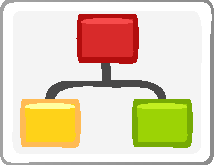
\includegraphics[scale=1.9]{img/diagram.pdf}
    \label{fig:diagram}
    \source{Extracted from \cite{larcc}.}
\end{figure}

\cite{GRIEBLER:IJPP:18}


\cite{MACCOOL:structured_patterns:book:12}


\section{Related Work}\label{sec:rw}


\tablename~\ref{tab:my_table} present an example of a Latex table.

\begin{table}[htb]
    \caption{This is a simple example to build a table.}
    \label{tab:my_table}
    \centering
    \begin{tabular}{|c|c|c|c|}
        \hline
         A & B & N & T\\ 
         \hline
         X & y & W & G\\
         \hline
    \end{tabular}
    
\end{table}
% Chapter 3
\chapter{Results}\label{chap:Results}

The experiments and developement goes here...

\section{History and Presentaion of the Organization}


\section{Developements} \label{sec:dev}


\lstlistingname~\ref{lst:python-code} presents a Python code example.

\begin{lstlisting}[numbers=left, language=Python, style=mycode, caption={Python code example.}, label={lst:python-code}]
import numpy as np
 
def incmatrix(genl1,genl2):
    m = len(genl1)
    n = len(genl2)
    M = None #to become the incidence matrix
    VT = np.zeros((n*m,1), int)  #dummy variable
 
    #compute the bitwise xor matrix
    M1 = bitxormatrix(genl1)
    M2 = np.triu(bitxormatrix(genl2),1) 
 
    for i in range(m-1):
        for j in range(i+1, m):
            [r,c] = np.where(M2 == M1[i,j])
            for k in range(len(r)):
                VT[(i)*n + r[k]] = 1;
                VT[(i)*n + c[k]] = 1;
                VT[(j)*n + r[k]] = 1;
                VT[(j)*n + c[k]] = 1;
 
                if M is None:
                    M = np.copy(VT)
                else:
                    M = np.concatenate((M, VT), 1)
 
                VT = np.zeros((n*m,1), int)
 
    return M
\end{lstlisting}

\lstlistingname~\ref{lst:cpp-code} presents a C++ code example.

% this is an example including from a file
\lstinputlisting[numbers=left,language=C++,style=mycode,caption={C++ code example.},label={lst:cpp-code}]{code/code-example.cpp}


\section{Experiments} \label{sec:exp}




\chapter*{Conclusions} \label{chap:concl}


Conclusions goes here ...





%\bibliographystyle{template/abnt}
%% para português
\bibliographystyle{template/abnt-pt}
\bibliography{bib/bibliography}




\end{document}